\mysection{ОБЗОР ПЛАТФОРМЫ ДЛЯ РАЗРАБОТКИ И~ПРОЕКТИРОВАНИЕ ВЕБ-ПРИЛОЖЕНИЯ}

\subsection{Платформа для разработки}
\label{subsec:reach-and-reachrs}

Разработка приложения будет осуществляться на платформе продуктов компании Emlid \cite{Emlid}: ГНСС модуля Reach \cite{Reach} и~ГНСС приёмника Reach~RS \cite{ReachRS}. Основой данных устройств являются вычислительный модуль Intel Edison и~плата, на которую установлен ГНСС модулю компании u-blox. Intel Edison работает под управлением GNU/Linux, что позволяет использовать многочисленные средства разработки, доступные для дистрибутивов данной операционной системы. \par

При разработке приложения на платформе указанных выше устройств важно учитывать следующий факт: несмотря на то, что Reach и~Reach~RS созданы на базе одного и~того же вычислительного модуля и~используют одинаковые приёмники u-blox, имеется ряд существенных различий в~аппаратном обеспечении данных устройств \cite{Reach, ReachRS}. Различия Reach и~Reach~RS, которые необходимо учесть при создании веб-приложения, указаны в~таблице \ref{tab:reach-vs-reachrs}.

\ctable[
  pos=h!,
  caption={Различия Reach и~Reach~RS},
  label={tab:reach-vs-reachrs}
]{|l|*{2}{>{\centering\arraybackslash}m{2.3cm}|}}{}{
  \toprule
  \multicolumn{1}{|c|}{\textbf{Техническая/функциональная особенность}} & \textbf{Reach} & \textbf{Reach~RS} \\
  \midrule
  Встроенная батарея & нет & да \\
  \midrule
  Встроенная антенна & нет & да \\
  \midrule
  Встроенное радио & нет & да \\
  % \midrule
  % Физическая кнопка на корпусе & нет & да \\
  \midrule
  Возможность управления фотокамерой & да & нет \\
  \bottomrule
}

Наличие (отсутствие) тех или иных возможностей у~Reach или Reach~RS отразится на клиентской части разрабатываемого решения в~виде специфических форм и~элементов интерфейса, отображение которых будет зависеть от того, на каком из устройств запущено приложение.

\subsection{Общая архитектура приложения}
\label{subsec:raw-app-architecture}

\subsubsection{Задачи и~требования}
\label{subsec:app-requirements}

Для создания общей архитектуры приложения необходимо определить наиболее важные идеи, задачи и~требования, предъявляемые к~разрабатываемому продукту. \par

Важно отметить, что в~следующем далее списке присутствуют пункты, которые касаются лишь разработчиков программных компонентов, отвечающих за взаимодействие с~RTKLIB, системными утилитами и~различными аппаратными компонентами Reach и~Reach~RS. Данные модули и~детали их разработки выходят за рамки рассматриваемой работы, но являются чрезвычайно важными для понимания общей структуры приложения. \par

Разрабатываемое приложение должно:

\begin{dashitemize}
  \item \textbf{Осуществлять запуск приложений RTKLIB в~управляемых контейнерах}. Надёжным и~простым способом организации взаимодействия с~приложениями RTKLIB является их запуск в~управляемых контейнерах. При данном подходе необходимые утилиты будут работать так же, как если бы пользователь запускал их в~терминале. \par

  Используя подобный подход, становится возможно организовать взаимодействие веб-приложения с~необходимыми программами таким образом, что:

  \begin{dashitemize}
    \item не требуется вмешательство в~исходный код RTKLIB;
    \item облегчается поддержка совместимости с~новыми версиями программного комплекса;
    \item разрабатываемый продукт остаётся независим от изменений в~кодовой базе RTKLIB. 
  \end{dashitemize}

  \item \textbf{Иметь клиентскую часть, представленную в~виде одностраничного приложения}. Основываясь на выводах, сделанных в~разделе 1, было принято решение реализовать клиентскую часть разрабатываемого решения в~виде одностраничного приложения. \par

  Как показал проведённый обзор, данный подход в~настоящее время является одним из самых популярных решений для создания веб-интерфейсов, предназначенных для управления такими устройствами, как Reach или Reach~RS.

  \item \textbf{Поддерживать передачу данных по протоколу WebSocket}. Для создания отзывчивого интерфейса веб-приложения и~обеспечения лучшего пользовательского опыта б\`{о}льшую часть взаимодействий клиентской части с~сервером следует организовать с~помощью асинхронных запросов и~сообщений. \par

  Наиболее удачным решение для разрабатываемого приложения является протокол WebSocket. Создавая на клиентской части веб-приложения слушателей определённых событий, становится возможно организовать отображение различной информации в~режиме реального времени без постоянных опросов сервера.
\end{dashitemize}

\subsubsection{Основные модули}
\label{subsec:app-modules}

Перечислим основные модули приложения (рис.~\ref{fig:raw-system-architecture}):

\begin{alphitemize}
  \item Серверная часть
  \begin{alphitemize}
    \item WebSocket сервер
    \item Модуль взаимодействия с~RTKLIB
    \item Демоны и~сервисы для взаимодействия с~аппаратными компонентами устройства
  \end{alphitemize}

  \item Клиентская часть
  \begin{alphitemize}
    \item WebSocket клиент
    \item JavaScript-приложение
  \end{alphitemize}
\end{alphitemize}

\begin{figure}[h!]
  \centering
  \setlength{\fboxsep}{5pt}
  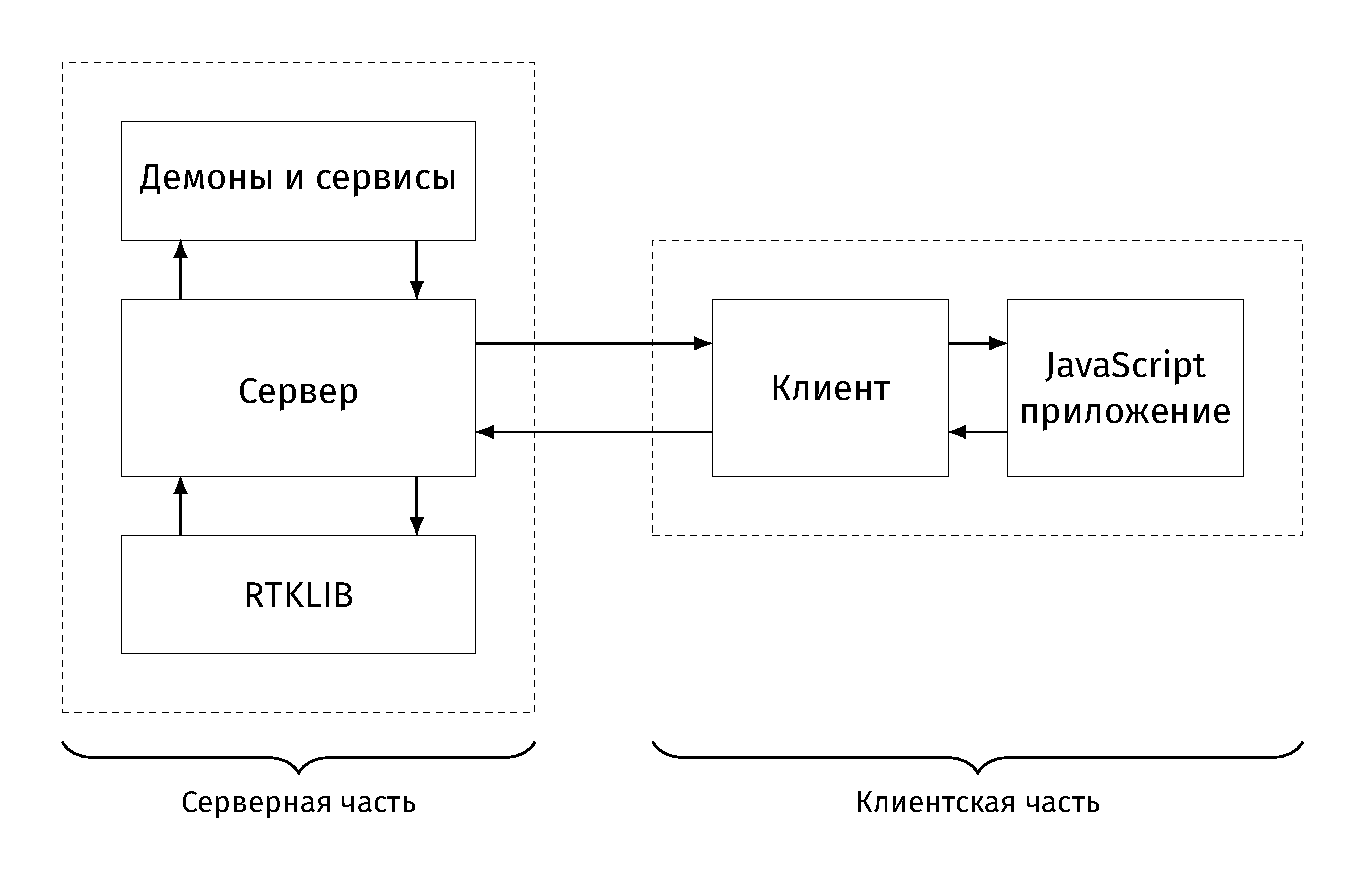
\includegraphics[width=.9\textwidth]{img/tikz/raw-system-architecture/pic}
  \vspace*{12pt}
  \caption{Общая архитектура приложения}\label{fig:raw-system-architecture}
\end{figure}

\subsection{Выбор инструментов разработки}
\label{subsec:programming-tools}

\subsubsection{Серверная часть приложения}
\label{subsec:backend-tools}

В~рамках разработки описанного приложения выбор инструментов для написания серверной части приложения зависит не только от возможностей веб-фреймворков, доступных для того или иного языка программирования, но и~от задач, описанных в~подразделе 2.2. Также, важно помнить, что разрабатываемое приложение предназначено для запуска на устройствах с~ограниченными вычислительными ресурсами. \par

Разработчиками серверной части приложения был проведён обзор высокоуровневых языков программирования, часто используемых для разработки веб-приложений. Основными из рассмотренных вариантов были такие популярные языки, как Java, Python, Ruby. \par

% TODO Оформить "переход" к списку наиболее важных библиотек/фреймворков
На основании различных оценок, детали формирования которых выходят за рамки рассматриваемой работы, основным языком для серверной части приложения был выбран Python.

\begin{dashitemize}
  \item Веб-фреймворк Flask
  \item pexpect
  \item GeoPandas
\end{dashitemize}

\subsubsection{Клиентская часть приложения}
\label{subsec:frontend-tools}

\paragraph{Основные средства}

Основу клиентской части приложения составят: язык гипертекстовой разметки HTML, CSS-стили и~скрипты на языке JavaScript.

Для наиболее быстрой и~удобной разработки одностраничного приложения было решено использовать специализированную библиотеку или фреймворк. На момент проектирования приложения одними из самых популярных [?] инструментов для создания одностраничных приложений являлись React [?], Angular 2 [?], Vue.js [?] и~Knockout [?].

Для анализа и сравнения вышеперечисленных библиотек и фреймворков были изучены:
\begin{dashitemize}
  \item официальные документации;
  \item исходные коды простейших приложений и~их компонентов;
  \item результаты синтетических тестов [?].
\end{dashitemize}

По результатам изучения возможных решений для разработки приложения был выбран фреймворк Vue.js. Данный выбор обусловлен не только плюсами фреймворка, выделенными во время анализа, но также наличием у автора данной работы опыта разработки с~использованием фреймворка AngularJS, который является одним из источников вдохновения для создателей Vue.js [?].

Также, вместе с~Vue.js было решено использовать библиотеку-расши-рение для данного фреймворка -- Vuex [?]. Данная библиотека позволит создать централизованное хранилище данных, доступ к~которому будут иметь все компоненты приложения. Одной из важнейших особенностей работы с~таким хранилищем является способность компонентов Vue.js реактивно обновлять своё состояние при изменении тех или иных данных в~Vuex.

% https://github.com/krausest/js-framework-benchmark
% http://www.stefankrause.net/js-frameworks-benchmark5/webdriver-ts/table.html
% http://www.stefankrause.net/js-frameworks-benchmark6/webdriver-ts-results/table.html

\paragraph{Работа с картами}

В качестве решения для задачи отображения карт и всевозможной информации на картах был выбран проект OpenLayers [?]. Данная библиотека предоставляет широкие возможности для работы с картами:
\begin{dashitemize}
  \item выбор источника графических тайлов карты;
  \item управление отображением элементов управления картой;
  \item модификация способов взаимодействия пользователя с картой;
  \item координатная сетка и шкала масштаба, доступные по умолчанию;
  \item возможность отрисовки произвольных фигур и изображений на различных слоях карты.
\end{dashitemize}

\paragraph{WebSockets}

Для работы с~WebSocket была выбрана библиотека Socket.IO [?]. Данный выбор обусловлен не только популярностью библиотеки, но и~наличием полной поддержки Socket.IO на серверной части приложения -- для веб-фреймворка Flask существует расширение Flask-SocketIO, позволяющее серверу обмениваться сообщениями с~любыми клиентами Socket.IO.


\subsection{Детализированная архитектура приложения}
\label{subsec:app-architecture}

С~учётом инструментов, выбранных в~предыдущем подразделе, уточним архитектуру приложения, представленную ранее (рис.~\ref{fig:raw-system-architecture}). На рисунке \ref{fig:complete-system-architecture} изображена детализированная архитектура разрабатываемого приложения.

\begin{figure}[h!]
  \centering
  \setlength{\fboxsep}{5pt}
  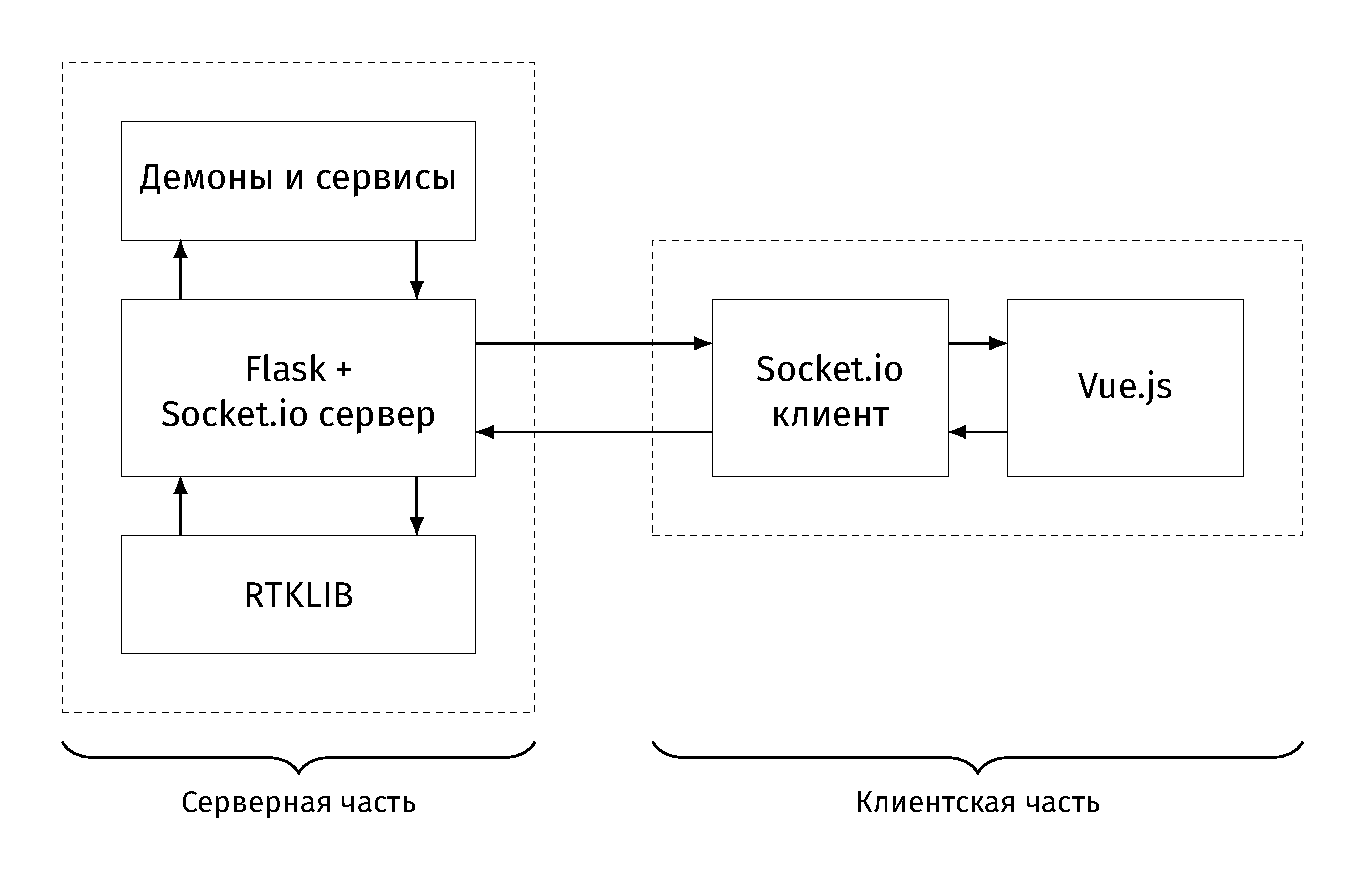
\includegraphics[width=.9\textwidth]{img/tikz/system-architecture/pic_sans_no-border}
  % \vspace*{12pt}
  \caption{Детализированная архитектура приложения}\label{fig:complete-system-architecture}
\end{figure}


\subsubsection{Подробная архитектура клиентской части приложения}
\label{subsec:frontend-architecture}

\begin{figure}[h!]
  \centering
  \setlength{\fboxsep}{5pt}
  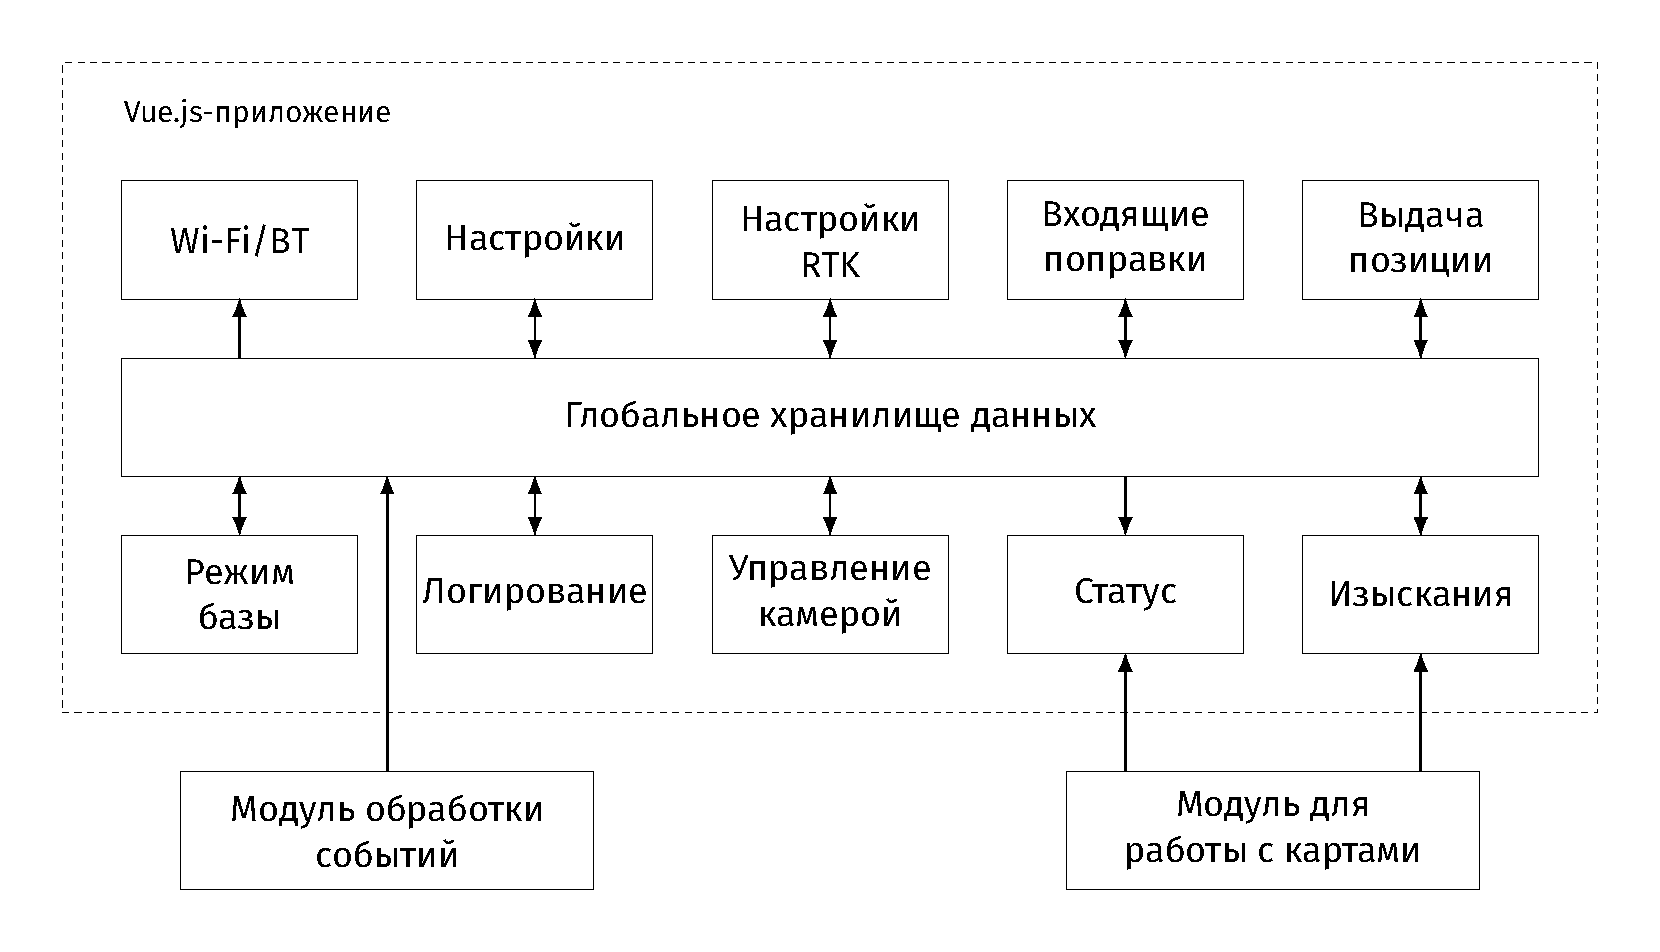
\includegraphics[width=\textwidth]{img/tikz/fe-architecture/pic}
  % \vspace*{12pt}
  \caption{Архитектура клиентской части приложения}\label{fig:fe-architecture}
\end{figure}


% \subsection{Функциональные требования к~модулям приложения}
\subsection{Описание модулей приложения и~основные требования, предъявляемые к~ним}
\label{subsec:app-modules-requirements}


\subsubsection{Статус}

Данный модуль служит для обработки, форматирования и~отображения основной информации, связанной с~работой приёмника:
\begin{dashitemize}
  \item значения отношений сигнал/шум (англ.~\emph{Signal-to-noise ratio, SNR}) для принимаемых со~спутников сигналов (для ровера и~базы);
  \item режим работы RTKLIB;
  \item качество получаемого решения;
  \item текущие координаты ровера;
  \item скорость движения ровера;
  \item параметры RTK;
  \item координаты базы.
\end{dashitemize}

Также, модуль должен осуществлять сбор и~хранение истории изменения координат ровера для отображения данной информации на интерактивной карте.


\subsubsection{Изыскания}

Модуль, реализующий инструменты для проведения полевых работ и~предоставляющий пользователю следующие возможности:
\begin{dashitemize}
  % TODO Необходимо ввести определение терминов "проект" и "точка"
  \item создание и~удаление проектов;
  \item экспорт проектов в~различных форматах;
  \item сбор и~вынос точек;
  \item просмотр данных проекта на интерактивной карте.
\end{dashitemize}

\paragraph{Создание проекта}

При создании нового проекта пользователь должен:
\begin{dashitemize}
  \item указать название проекта;
  \item указать имя автора проекта;
  \item добавить описание проекта (опционально);
  \item ввести высоту антенны по умолчанию;
  \item создать до трёх правил для автоматического сбора точек.
\end{dashitemize}

% TODO Ведь нужно использовать слово "осреднение", верно?
Правила для автоматического сбора точек представляют собой условия, при которых устройство автоматически будет принимать результаты осреднения координат. Параметры правил:
\begin{dashitemize}
  \item статус решения (Single, Float или Fix);
  \item минимальное время сбора (от одной секунды до одного часа);
  \item максимальное допустимое значение СКО;
  \item максимальное допустимое значение DOP.
\end{dashitemize}

\paragraph{Экспорт проекта}

Экспорт проектов должен быть доступен в следующих форматах:
\begin{dashitemize}
  \item GeoJSON;
  \item ESRI Shapefile;
  \item DXF;
  \item CSV;
  \item DroneDeploy CSV.
\end{dashitemize}


\subsubsection{Настройки RTK}

Модуль приложения, необходимый для настройки параметров RTK и~используемых ГНСС.

Настраиваемые параметры RTK:
\begin{dashitemize}
  \item режим позиционирования (Single, Static или Kinematic);
  \item метод разрешения фазовой неоднозначности;
  \item угол отсечки спутников (от 0 до 30 градусов);
  \item маска для отношения сигнал/шум (от 0 до 40);
  \item максимальные возможные горизонтальные и~вертикальные ускорения ГНСС-антенны (от 0 до 10 $\text{м/с}^{2}$).
\end{dashitemize}

% TODO Добавить параграфы?
Настройки используемых ГНСС:
\begin{dashitemize}
  \item выбор ГНСС из списка, представленного в~пункте \ref{subsec:rtklib-supported-gnss};
  \item выбор частоты обновления навигационных данных (1, 5, 10 или 14~Гц).
\end{dashitemize}

При настройке необходимо соблюдать следующие ограничения:
\begin{alphitemize}
  \item получение данных GPS невозможно отключить;
  \item \label{itm:glonass-beidou-conflict} невозможно одновременно включить системы ГЛОНАСС и~BeiDou;
  \item \label{itm:glonass-beidou-update-rates} невозможно настроить получение данных от ГЛОНАСС и~BeiDou при частоте обновления выше 5 Гц.
\end{alphitemize}

Ограничения, указанные в~пунктах \ref{itm:glonass-beidou-conflict} и~\ref{itm:glonass-beidou-update-rates} списка выше, обусловлены аппаратными ограничениями приёмника u-blox, установленного в~устройствах Reach и~Reach~RS.


\subsubsection{Входящие поправки}

Данный модуль необходим для настройки получения ровером поправок с~базы. В~список задач, решаемых данным компонентом, входит выбор способа получения поправок и~настройка значений, специфичных для каждого из них.

Способы получения поправок и~элементы их конфигурации:
\begin{dashitemize}
  \item последовательный порт
  \begin{dashitemize}
    \item устройство (UART, USB-to-PC, USB-OTG);
    \item скорость передачи (бод);
    \item формат данных.
  \end{dashitemize}

  \item NTRIP
  \begin{dashitemize}
    \item адрес;
    \item порт;
    \item имя пользователя (опционально);
    \item пароль (опционально);
    \item точка подключения;
    \item формат данных.
  \end{dashitemize}

  \item TCP соединение
  \begin{dashitemize}
    \item роль (сервер, клиент);
    \item адрес;
    \item порт;
    \item формат данных.
  \end{dashitemize}

  \item Bluetooth
  \begin{dashitemize}
    \item формат данных.
  \end{dashitemize}

  \item LoRa
  \begin{dashitemize}
    \item частота;
    \item выходная мощность;
    \item битрейт;
    \item формат данных.
  \end{dashitemize}
\end{dashitemize}


\subsubsection{Выдача позиции}

Модуль, позволяющий настроить до двух потоков данных, содержащих информацию о~текущей позиции устройства. Как и~в~случае с~настройкой входящих поправок, рассматриваемый модуль предоставляет инструменты для выбора способа передачи данных и~их конфигурации.

Способы передачи данных и~элементы их конфигурации:
\begin{dashitemize}
  \item последовательный порт
  \begin{dashitemize}
    \item устройство (UART, USB-to-PC, USB-OTG);
    \item скорость передачи (бод);
    \item формат данных.
  \end{dashitemize}

  \item TCP соединение
  \begin{dashitemize}
    \item роль (сервер, клиент);
    \item адрес;
    \item порт;
    \item формат данных.
  \end{dashitemize}

  \item Bluetooth
  \begin{dashitemize}
    \item формат данных.
  \end{dashitemize}
\end{dashitemize}


\subsubsection{Режим базы}

Модуль, предназначенный для настройки параметров, специфичных для устройства, работающего в~режиме базы. Содержит в~себе инструменты для:
\begin{dashitemize}
  \item настройки потока данных с~поправками (способы и~их настройки);
  \item выбора типов передаваемых сообщений и~частоты их передачи;
  \item установки точных координат будущей базы (автоматически и~вручную).
\end{dashitemize}

Способы передачи данных и~элементы их конфигурации:
\begin{dashitemize}
  \item последовательный порт
  \begin{dashitemize}
    \item устройство (UART, USB-to-PC, USB-OTG);
    \item скорость передачи (бод);
    \item формат данных.
  \end{dashitemize}

  \item NTRIP
  \begin{dashitemize}
    \item адрес;
    \item порт;
    \item пароль (опционально);
    \item точка подключения.
  \end{dashitemize}

  \item TCP соединение
  \begin{dashitemize}
    \item роль (сервер, клиент);
    \item адрес;
    \item порт;
    \item формат данных.
  \end{dashitemize}

  \item Bluetooth
  \begin{dashitemize}
    \item формат данных.
  \end{dashitemize}

  \item LoRa
  \begin{dashitemize}
    \item частота;
    \item выходная мощность;
    \item битрейт;
    \item формат данных.
  \end{dashitemize}
\end{dashitemize}

При настройке устройства в~режиме базы необходимо соблюдать следующие ограничения:
\begin{dashitemize}
  % TODO Написать нормально
  \item объём сообщений при выборе LoRa;
  \item валидация координат.
\end{dashitemize}


\subsubsection{Логирование}

Данный модуль необходим для управления записью и~историей логов данных. Модуль решает следующие задачи:
\begin{dashitemize}
  \item включения (выключения) записи и~выбор формата логов определённого типа;
  \item получение списка доступных логов.
\end{dashitemize}


% центральный синхроконтакт
\subsubsection{Управление камерой}

Модуль, позволяющая произвести настройку управления камерой для осуществления аэрофотосъёмки. Данная возможность доступна только для устройств Reach.


% TODO Вкладка может быть разделена две
\subsubsection{Wi-Fi/Bluetooth}

Модуль управления беспроводными соединениями, позволяющий настраивать подключения в~Wi-Fi сетям, управлять работой устройства в~режиме точки доступа, а~также производить подключение к~различным устройствам по Bluetooth.


\subsubsection{Настройки}

Модуль, содержащий инструменты для общей настройки устройства (имя устройства, канал получения обновлений и~т.д.) и~различные утилитарные возможности (сброс настроек, генерирование системных отчётов).


\subsubsection{Модуль событий}

Модуль служит для регистрации слушателей событий, данные которых необходимы для множества модулей или для всего приложения в целом.


\subsubsection{Модуль работы с картами}

Данный модуль представляет собой обёртку над библиотекой OpenLayers. Наличие подобного компонента в приложении обусловлено необходимостью быстро и удобно создавать интерактивные карты для различных экранов приложения.

Модуль должен предоставлять конструктор для создания нового экземпляра карты OpenLayers. Единственным необходимым параметром конструктора должен быть уникальный идентификатор DOM-элемента, в котором будет отображена карта. В качестве дополнительного параметра конструктор должен принимать объект конфигурации, который позволит:
\begin{dashitemize}
  \item включить (отключить) отображение координатной сетки;
  \item настроить отображение элементов управления картой, добавленных по умолчанию;
  \item включить (отключить) различные типы взаимодействий с картой.
\end{dashitemize}


\subsubsection{Общие замечания и~ограничения, накладываемые модули, предназначенные для конфигурации устройства}

\begin{dashitemize}
  \item ограничения на порты TCP-серверов;
  \item Bluetooth IO conflict;
  \item LoRa is only for RS;
  \item LoRa IO conflict;
  \item LoRa local constraints;
  \item Serial IO warnings.
\end{dashitemize}


\subsection{Создание макета веб-приложения}
\label{subsec:app-sketch}

\subsubsection{Общий вид приложения}
\label{subsec:app-sketch-general}

На основе наблюдений, сделанных в~подразделе \ref{subsec:web-apps-review}, было принято решение разнести многочисленные функции приложения по отдельным вкладкам. Подобное разделение панелей индикаторов (англ.~\emph{dashboard}), всевозможных форм настроек и~прочих элементов управления призвано сделать интерфейс приложения интуитивным, а~процесс работы пользователя с~устройством -- комфортным.

Разделение интерфейса на вкладки, по сути, является отображением модульной структуры приложения, описанной в~подразделах \ref{subsec:app-architecture} и~\ref{subsec:app-modules-requirements}. Был сформирован следующий список вкладок, содержащих элементы управления, относящиеся только к~конкретной части приложения:

\begin{dashitemize}
  \item Статус (англ.~\emph{Status});
  \item Изыскания (англ.~\emph{Survey});
  \item Настройки RTK (англ.~\emph{RTK settings});
  \item Входящие поправки (англ.~\emph{Correction input});
  \item Выдача позиции (англ.~\emph{Position output});
  \item Режим базы (англ.~\emph{Base mode});
  \item Логирование (англ.~\emph{Logging});
  \item Управление камерой (англ.~\emph{Camera control});
  \item Wi-Fi/Bluetooth;
  \item Настройки (англ.~\emph{Settings}).
\end{dashitemize}

\subsubsection{Описание интерфейса отдельных вкладок приложения}
\label{subsec:app-sketch-tabs}

\begin{dashitemize}
  \item \textbf{Статус} (рис.~??)

  \item \textbf{Изыскания} (рис.~??)
  % В данном разделе приложения пользователь может получить доступ к интерфейсам сбора и выноса точек, а также к списку проектов, представляющих собой способ организации результатов геодезических изысканий.

  \item \textbf{Настройки RTK} (рис.~??)

  \item \textbf{Входящие поправки} (рис.~??).

  \item \textbf{Выдача позиции} (рис.~??)

  \item \textbf{Режим базы} (рис.~??)

  \item \textbf{Логирование}

  % центральный синхроконтакт
  \item \textbf{Управление камерой} (рис.~??)

  % TODO Вкладка может быть разделена две
  \item \textbf{Wi-Fi/Bluetooth} (рис.~??)

  \item \textbf{Настройки} (рис.~??)
\end{dashitemize}

\newpage
